\documentclass[tikz,border=2pt]{standalone}
\usepackage{amsmath,amssymb}
\usepackage{tikz}
\usetikzlibrary{arrows.meta}

\begin{document}
% One realisation of a Poisson process: arrivals at random times (crosses on the time axis)
% and the counting process N_t, which jumps by one at each arrival.
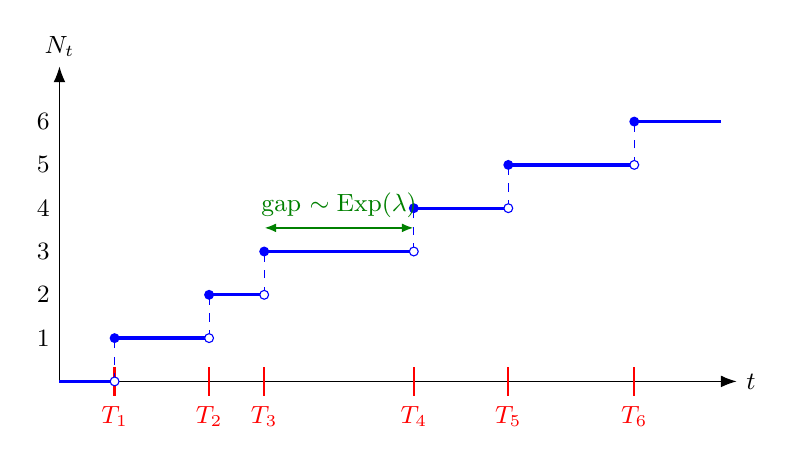
\begin{tikzpicture}[every node/.style={font=\small}, >={Latex[length=2mm]}]
	\draw[->] (0,0) -- (8.6,0) node[right] {$t$};
	\draw[->] (0,0) -- (0,4.0) node[above] {$N_t$};
	\foreach \y in {1,...,6} {\node[left, font=\small] at (0,{\y*0.55}) {\y};}
	\foreach \t in {0.7,1.9,2.6,4.5,5.7,7.3} {\draw[red, thick] (\t,-0.18) -- (\t,0.18);}
	\node[red, font=\small, anchor=north] at (0.7,-0.2) {$T_1$};
	\node[red, font=\small, anchor=north] at (1.9,-0.2) {$T_2$};
	\node[red, font=\small, anchor=north] at (2.6,-0.2) {$T_3$};
	\node[red, font=\small, anchor=north] at (4.5,-0.2) {$T_4$};
	\node[red, font=\small, anchor=north] at (5.7,-0.2) {$T_5$};
	\node[red, font=\small, anchor=north] at (7.3,-0.2) {$T_6$};
	\draw[blue, very thick] (0,0) -- (0.7,0);
	\draw[blue, very thick] (0.7,0.55) -- (1.9,0.55);
	\draw[blue, very thick] (1.9,1.1) -- (2.6,1.1);
	\draw[blue, very thick] (2.6,1.65) -- (4.5,1.65);
	\draw[blue, very thick] (4.5,2.2) -- (5.7,2.2);
	\draw[blue, very thick] (5.7,2.75) -- (7.3,2.75);
	\draw[blue, very thick] (7.3,3.3) -- (8.4,3.3);
	\foreach \t/\y in {0.7/0.55, 1.9/1.1, 2.6/1.65, 4.5/2.2, 5.7/2.75, 7.3/3.3} {
		\draw[blue, dashed] (\t,{\y-0.55}) -- (\t,\y);
		\fill[blue] (\t,\y) circle (1.8pt);
		\draw[blue, fill=white] (\t,{\y-0.55}) circle (1.6pt);
	}
	\draw[{Latex[length=1.5mm]}-{Latex[length=1.5mm]}, green!50!black, thick] (2.6,1.95) -- (4.5,1.95) node[midway, above, font=\small] {gap $\sim\operatorname{Exp}(\lambda)$};
	
\end{tikzpicture}
\end{document}
